\textcolor[rgb]{0.00,0.00,1.00}{In this section we briefly recall the regression trees-based control algorithm proposed in \cite{Behl201630} for the DR control problem, i.e. mbCRT. In particular, we will provide a more general formulation that is suitable for generic cyber-physical systems. This will be useful in the next section to introduce our new methodology. In particular, we first state the strategy used to construct data-driven cyber-physical system models using regression trees. Secondly, we setup a optimal control problem that is based on such models.}

\subsection{Data-based one step lookahead predictive model}
\label{sec:mbcrt}

\begin{figure}
\centering
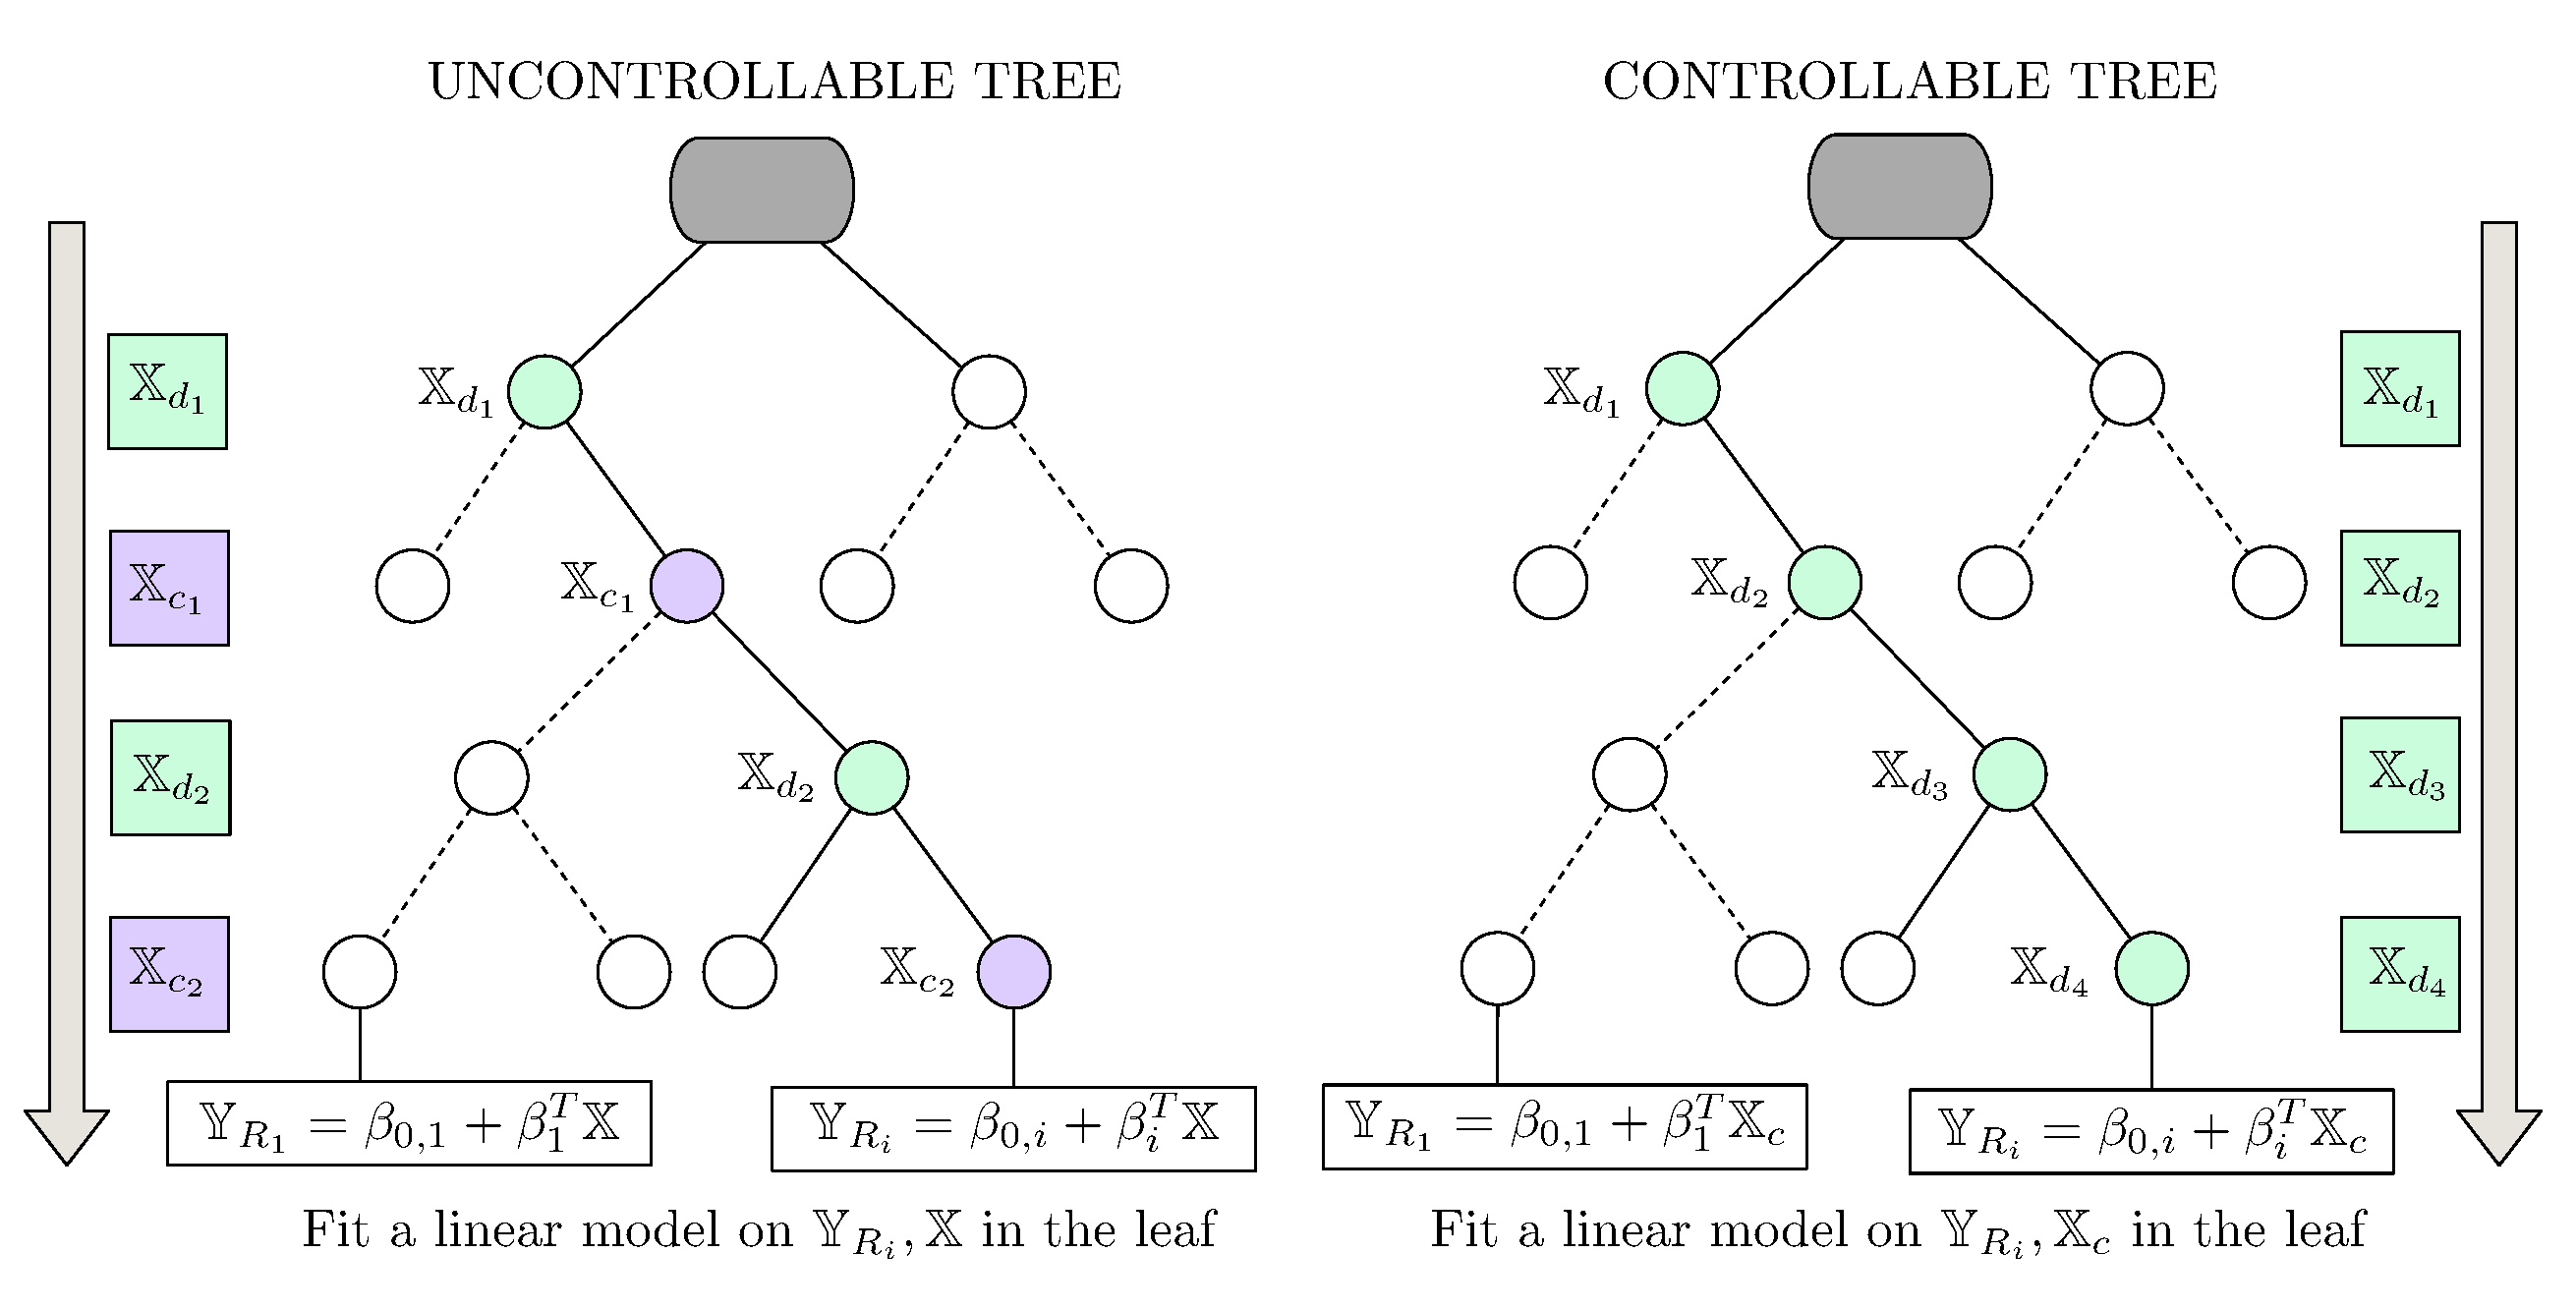
\includegraphics[width=0.95\columnwidth]{Figures/sep_vars.eps}
   \caption{Example of a regression tree not suitable for control due to the mixed order of $\mathcal{X}_c$ and $\mathcal{X}_d$ (left). Example of a tree structure obtained used for mbCRT algorithm. The separation of variables allows using the linear model in the leaf to use only control variables (right).}
   \captionsetup{justification=centering}
   \label{fig:training}
\end{figure}

%\begin{figure}
%	\centering
%	\subfigure{
%		\label{F:RT}
%		\centering
%		\begin{tikzpicture}[->,>=stealth',level/.style={sibling distance = 3.5cm/#1,
%			level distance = 1.5cm}] 
%		\node [branch_c] {}
%		child[blue!50!gray!,thick]{ node [branch_l] {}
%			child[blue!50!gray!,thick]{ node [branch_l] {$R_1$} edge from parent node[above left] {$\u_j \leq t_j$}}
%			child[red!50!gray!,thick]{ node [branch_r] {$R_2$} edge from parent node[above right] {$\u_j> t_j$}} 
%			edge from parent node[above left] {$\mathrm{d}_i \leq t_i$}                            
%		}
%		child[red!50!gray!,thick]{ node [branch_r] {}
%			child[blue!50!gray!,thick]{ node [branch_l] {}
%				child[blue!50!gray!,thick]{ node [branch_l] {$R_4$} edge from parent node[above left] {$\mathrm{d}_k \leq t_k$}}
%				child[red!50!gray!,thick]{ node [branch_r] {$R_5$} edge from parent node[above right] {$\mathrm{d}_k > t_k$}} 
%			}
%			child[red!50!gray!,thick]{ node [branch_r] {$R_3$}}  
%			edge from parent node[above right] {$\mathrm{d}_i> t_i$}    
%		}
%		; 
%		\end{tikzpicture}
%	}
%	\subfigure{
%		\label{F:RT2}
%		\centering
%		\begin{tikzpicture}[->,>=stealth',level/.style={sibling distance = 3.5cm/#1,
%			level distance = 1.5cm}] 
%		\node [branch_c] {}
%		child[blue!50!gray!,thick]{ node [branch_l] {}
%			child[blue!50!gray!,thick]{ node [branch_l] {$R_1$} edge from parent node[above left] {$\mathrm{d}_j \leq t_j$}}
%			child[red!50!gray!,thick]{ node [branch_r] {$R_2$} edge from parent node[above right] {$\mathrm{d}_j > t_j$}} 
%			edge from parent node[above left] {$\mathrm{d}_i \leq t_i$}                            
%		}
%		child[red!50!gray!,thick]{ node [branch_r] {}
%			child[blue!50!gray!,thick]{ node [branch_l] {}
%				child[blue!50!gray!,thick]{ node [branch_l] {$R_4$} 
%					child[blue!50!gray!,thick]{ node [branch_l] {} edge from parent node[above] {}}}
%				child[red!50!gray!,thick]{ node [branch_r] {$R_5$} edge from parent node[above right] {$\mathrm{d}_k > t_k$}}
%			}
%			child[red!50!gray!,thick]{ node [branch_r] {$R_3$}}  
%			edge from parent node[above right] {$\mathrm{d}_i> t_i$}    
%		}
%		; 
%		\end{tikzpicture}
%	}
%	\caption{Example of a regression tree not suitable for control due to the mixed order of $\mathcal{X}_c$ and $\mathcal{X}_d$ (left). Example of a tree structure obtained used for mbCRT algorithm. The separation of variables allows using the linear model in the leaf to use only control variables (right).}
%	\captionsetup{justification=centering}
%\end{figure}

\textcolor[rgb]{0.00,0.00,1.00}{Using this separation of variables introduced in Sec. \ref{sec:problem}, \emph{model based Control with Regression Trees (mbCRT)} is built upon the idea of simple model based regression trees~\cite{friedman1991multivariate}. In particular, as already hinted at Sec. \ref{sec:problem} and as illustrated in the right part of Fig. \ref{fig:training}, a regression tree is trained only on disturbance features in $\mathcal{X}_d= \{ \mathrm{d_1,\ldots,d_{s-m}} \} $ to predict the output variable $\mathrm{y}$. Without any loss of generality, here we consider only $1$ response variable, but multiple trees can be considered for multiple response variables as we do for the case study in Sec. \ref{sec:case}. After the regression tree partitioning, a linear model is fitted using the subset of samples present in the leaf $R_i$}

\textcolor[rgb]{0.00,0.00,1.00}{\begin{equation}\label{eq:linear_regression_leaf}
\mathrm{y}_{R_i} = \beta_{0,i} + \beta_i u
\end{equation}
where $\mathrm{y}_{R_i}$ is the predicted response in region $R_i$ of the tree using all the features in $\mathcal{X}_d$, and $\beta_{0,i}\in\mathbb{R}$ and $\beta_i\in\mathbb{R}^{1\times m}$. Separation of variables allows to use the forecast of the disturbances in $\mathcal{X}_d$ to navigate to the appropriate region $R_i$ and use the linear regression model \eqref{eq:linear_regression_leaf} with only the control variables in it as the valid prediction model for that time-step. Left part of Fig. \ref{fig:training} shows the case where all the features in $\mathcal{X}$ are used to train the trees. As one can see, control variables are used to create several split in the tree. As a consequence, as already explained in Sec. \ref{sec:problem} this does not allow to set up a MPC-like optimization problem, since inputs values are not available a priori to go through the tree and determine the correct region $R_i$.}

\subsection{Data-based optimal control}
\textcolor[rgb]{0.00,0.00,1.00}{Given $p$ response variables and $s$ training features, of which $m$ input and $s-m$ disturbance variables, $p$ regression trees are built to create models as in \eqref{eq:linear_regression_leaf} for every response variable. Then at each time-step $t$ the following quadratic optimal control problem is solved}

\textcolor[rgb]{0.00,0.00,1.00}{
\begin{equation}\label{eq:mbCRT}
\begin{aligned}
& \underset{u_t \in \mathcal{X}_c}{\text{minimize}} & &  y^\top_t \mathrm{Q}\, y_t + u^\top_t \mathrm{R}\, u_t              \\
& \text{subject to }                                & &  \mathrm{y}_{1,t}    =   \beta_{0,i_1} + \beta_{i_1}u_t     \\
&                                                   & &  \mathrm{y}_{2,t}    =   \beta_{0,i_2} + \beta_{i_2}u_t     \\
&                                                   & &  \vdots                                                         \\
&                                                   & &  \mathrm{y}_{p,t}    =   \beta_{0,i_p} + \beta_{i_p}u_t     \\
&                                                   & &  u_t                \in  \mathcal{\bar U}                       \\
\end{aligned}
\end{equation}
Only the first the optimal control input $u(t) = u^*_t$ is applied to the system, then the algorithm is repeated at $t+1$, and so on. $\mathrm{Q}$ and $\mathrm{R}$ are design parameters to trade-off the quadratic objective function components. Different objective functions can be chosen, for example linear or non-linear, as well as different models in the leaves instead of \eqref{eq:linear_regression_leaf}, so decreasing or increasing the complexity of the problem. The good quality of the linear model approximation has been already shown in \cite{Behl201630}.}
